\documentclass{bioinfo}
\copyrightyear{2014}
\pubyear{2014}

\begin{document}
\firstpage{1}

\title[dnaplotlib]{dnaplotlib: visualization of genetic constructs, libraries and associated data}
\author[Thomas E. Gorochowski \textit{et~al.}]{Thomas~E.~Gorochowski$^{1,\dagger}$, Bryan~Der$^{1,\dagger}$, Emerson~Glassey$^{1,\dagger}$, D. Benjamin Gordon$^{1}$ and Christopher~A.~Voigt$^{1,}$\footnote{to whom correspondence should be addressed}}
\address{$^{1}$Department of Biological Engineering, Synthetic Biology Center, Massachusetts Institute of Technology, USA.\\
$^{\dagger}$These authors contributed equally to this work.}


\history{Received on XXXXX; revised on XXXXX; accepted on XXXXX}

\editor{Associate Editor: XXXXXXX}

\maketitle

\begin{abstract}

\section{Summary:}
dnaplotlib is a computational toolkit that enables highly customizable visualization of individual genetic constructs and libraries of design variants. Publication quality vector-based output is produced and all aspects of the rendering process can be easily customized or replaced by the user. dnaplotlib is capable of SBOL Visual compliant diagrams in addition to a format able to better illustrate the precise location and length of each genetic part. This alternative visualization method enables direct comparison with nucleotide-level information such as RNA-seq read depth. While it is envisaged that access will be predominantly via the programming interface, a web interface is also provided to support broader usage.

\section{Availability:}
dnaplotlib is cross-platform and open-source software developed using Python and released under the OSI recognised NPOSL-3.0 licence. Source code, documentation and a web front-end are available at the project website: \href{http://www.dnaplotlib.org}{http://www.dnaplotlib.org}.

\section{Contact:} \href{cavoigt@gmail.com}{cavoigt@gmail.com}
\end{abstract}

% 1. (1 para). Introduction to the need for standardized visualization of genetic designs. Sell the approach.
Engineering disciplines rely on the use of standards to clearly communicate design information and allow for the contruction of large and complex systems. As synthetic biology 

Attempts have been made to visualize conceptual genetic designs 
To date limited attempts have been made to aid in the visualization of conceptual genetic designs \citep{Bhatia13a} and although many DNA design tools offer the ability to . Firstly, output is generally 
The biggest limitation of these approaches so far though is an inability to integrate with existing scientific computing visualization and analysis tools. This is essential as 

% 2. (1 para). Existing tools that are available and the current difficulties in using them, e.g., PigeonCAD \citep{Bhatia13a}. Why is it needed... difficulty with library designs \citep{Smanski14a,Bilitchenko11a}.

% 3. (3 para). What dnaplotlib is: Python-based, uses matplotlib \citep{Hunter07a}, generates publication quality vector-based output. Highly customizable at all stages of the rendering process. Enables both single and libraries to be easily visualized. Describe the rendering pipeline (should tie into figure), and multiple types of output available.

To address these needs dnaplotlib has been built using matplotlib \citep{Hunter07a}, a Python-based 2D graphics library. This library is highly portable and allows for output in the form of vector based PDFs or rasterised PNG or JPEG images, as well as easy integration into existing plotting functionality. Python was chosen due to its increasing use for the analysis of biological data \citep{Cock09a} and its availability across all major operating systems.

A key consideration in the design of dnaplotlib was ensuring all aspects of the rendering process could be customized to user requirements. As fields such as synthetic biology are still evolving, the the precise way in which such tools will be used and the discovery of new types of genetic part that need to be included, but may not yet have a standardized representation. Enabling custom elements to be easily added and refined over time will ensure such elements are captured and also contribute to the standardization process. 

To generate a 

In addition to direct library access through Python analysis scripts, we also provide two scripts to enable input in the form of text files

% 4. (1 para). Web-based interface. What does this include, what it doesn't. Why did we make it.

To ensure broadest application of these tools that included use by non-programmers, we also developed a web-based interface that allows text files describing part styles and DNA designs to be uploaded and processed. These files uploaded to the server, processed by the scripts described previously, and generated images are returned to the user. This ensures broadest use of the library and ensures that members across a lab can share the same styling of diagrams to ensure clear communication of their designs.

We see a key feature of ensuring adoption as 

% 5. (1 para). Broader view. How is this toolkit going to help the community. Broader use of SBOL-compliant figures? Easier communication of ideas. Still able to have a lab ``style'' to differentiate your work and emphasize aspects in unique ways.

As synthetic biology moves ever closer to automated design procedures that harness the potential to construct huge libraries of design variants \citep{Smanski14a,Bilitchenko11a}, supporting visualization tools will become important to ensure clear communication of these large and diverse designs. The SBOL Visual initiative was started to aid in this task with the definition of agreed pictorial representations of genetic elements \citep{Quinn13a}. However, so far it has seen limited uptake due to a lack a tools that are able to be easily integrated into existing analysis workflows. dnaplotlib fills this gap by providing a computational toolkit that both adheres to this standard while also enabling highly customizable visualizations that are most appropriate for the specific needs of the laboratory. It is hoped that by providing researchers with this flexibility that they will be more willing to apply such standards to their work, improving general uptake of SBOL Visual across the field.

\begin{figure*}[t]
\centering
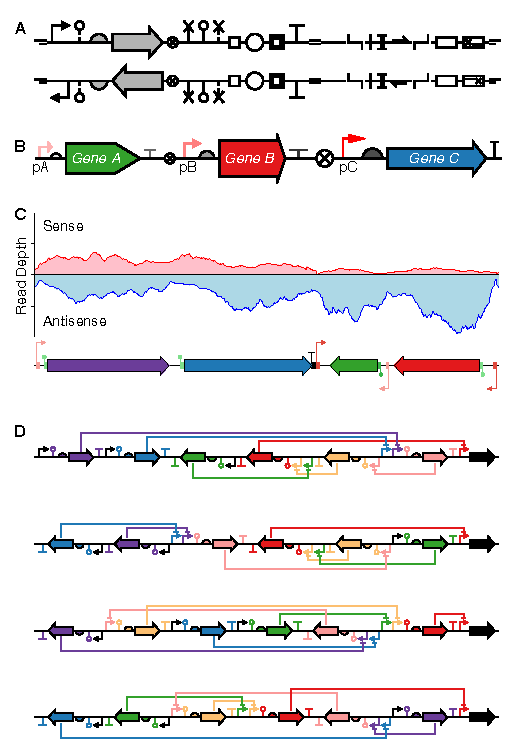
\includegraphics[width=\textwidth]{Figure1.pdf}
\caption{\label{fig:overview}Overview of the dnaplotlib library. (a) General architecture and currently available interfaces. (b) The full set of SBOL Visual parts is available in forward (top) and reverse (bottom) orientations. Size, colour and shape of all these elements can be easily customized to a users requirements. (c) To allow for direct comparison between designs and nucleotide data such as RNA-seq read depths, we offer trace-based renderers where part correct widths are aligned to the trace. (d) Example library of the potential genetic design variants implementing the same 3-input (black promoters), 1-output (black CDS) device. Colour is used to link repressor genes to their cognate promoter.}
\end{figure*}

% 6. (1 para). Future directions (general point on where it is available and contributions)

dnaplotlib is under continual development with a current focus on broadening the types of genetic element covered to include new synthetic biological parts. The project welcomes contributions from others within the community through the project website and public development repository at: \href{http://www.dnaplotlib.org}{http://www.dnaplotlib.org}.

\section*{ACKNOWLEDGEMENTS}
T.E.G. was supported by TODO. E.G. was supported by TODO. B.D. was supported by TODO. C.A.V. was supported by TODO.

\begin{thebibliography}{}
	
\bibitem[Bhatia \& Densmore, 2013]{Bhatia13a} Bhatia, S. and Densmore, D. (2013). Pigeon: A Design Visualizer for Synthetic Biology, {\it ACS Synth. Biol.}, {\bf 2}, 348-350.

\bibitem[Smanski {\it et~al}., 2014]{Smanski14a} Smanski, M.J., Swapnil, B., Park, YJ., Zhao, D., Giannoukos, G., Ciulla, D., Busby, M., Calderon, J., Nicol, R., Gordon, D.B., Densmore, D. and Voigt, C.A. (2014) Combinatorial design and assembly of refactored gene clusters, {\it Nat. Biotech.}, {\bf ?}, ???-???.

\bibitem[Hunter, 2007]{Hunter07a} Hunter, J.D. (2007). Matplotlib: A 2D graphics environment, {\it Computing in Science \& Engineering}, {\bf 9}, 90-95.

\bibitem[Cock {\it et~al}., 2009]{Cock09a} 
Cock PJ, Antao T, Chang JT, Chapman BA, Cox CJ, Dalke A, Friedberg I, Hamelryck T, Kauff F, Wilczynski B, and de Hoon MJ. (2009) Biopython: freely available Python tools for computational molecular biology and bioinformatics. {\it Bioinformatics}, {\bf 25}, 1422-1422.

\bibitem[Bilitchenko {\it et~al}., 2011]{Bilitchenko11a} 
Bilitchenko, L., Liu, A., Cheung, S., Weeding, E., Xia, B., Leguia, M., Anderson, J.C., Densmore, D. (2011) Eugene – A Domain Specific Language for Specifying and Constraining Synthetic Biological Parts, Devices, and Systems. {\it PLoS ONE}, {\bf 6}, e18882.

\bibitem[Quinn {\it et~al}., 2013]{Quinn13a} 
Quinn, J., Beal, J., Bhatia, S., Cai, P., Chen, J., Clancy, K., Hillson, N., Galdzicki, M., Maheshwari, A.P., Umesh; P., Matthew; R.C.; Stan, G.-B., Endy, D. (2013) ``Synthetic Biology Open Language Visual (SBOL Visual), version 1.0.0.''

\end{thebibliography}

\end{document}
